\documentclass[../main/main.tex]{subfiles}
\begin{document}

\chapter{The need of a non-perturbative approach}

We saw in the previous chapter that all the interesting physical quantities can be computed, both in high-energy physics and in condensed matter physics, using the perturbative approach. In this chapter we'll see why what we said doesn't really work so good, and in some instances we need a non-perturbative approach. We already anticipated some problems in the introduction, now we'll go more in details. 

\section{The asymptotic series}

\subsubsection{Divergent quantities}

Let's start from the simple example provided by a massive theory with quartic coupling in $d=0$. Consider the following quantity, which naturally emerges in perturbative computations:
\begin{eq}\label{eq:pert-probl-int1}
	\frac{\displaystyle \int\de x\,e^{-\frac\alpha2x^2}e^{-\lambda x^4}}{\displaystyle\int\de x\,e^{-\frac{\alpha}2x^2}}
	\tfor \lambda>0 \tcomma \Re\alpha>0
\end{eq}
Such quantity is clearly smaller than 1, since the numerator contains the integral of a function which is everywhere smaller than the function in the integral present in the denominator. Nevertheless if one applies the perturbative prescription, the previous quantity is substituted by 
\begin{eq}\label{eq:pert-probl-int2}
	\frac{\displaystyle\sum_{n=0}^\infty\frac1{n!}\int\de x\,e^{-\frac\alpha2x^2}(-\lambda x^4)^n}{\displaystyle\int\de x\,e^{-\frac{\alpha}2x^2}}
\end{eq}
But if one tries to compute explicitly the coefficient of the series
\begin{eq}
	\frac{\displaystyle\int\de x\,e^{-\frac\alpha2x^2}(\lambda x^4)^n}{\displaystyle\int\de x\,e^{-\frac{\alpha}2x^2}}
	=\lambda^n\frac{(4n)!}{(2n)!}\frac1{2^{2n+1}}\frac1{\alpha^{2n}}
	\geq \frac{\lambda^n}2\frac{((2n)!)^2}{(2n)!}\frac1{(2\alpha)^{2n}}
	=\frac{\lambda^n}2 \frac{(2n)!} {(2\alpha)^{2n}}
	\geq \frac12\left(\frac\lambda{(2\alpha)^2}\right)^n(n!)^2
\end{eq}
one gets that the series eq.~\eqref{eq:pert-probl-int2} is absolutely divergent
\begin{eq}
	\sum_{n=0}^\infty\left\vert\frac{(-\lambda)^n}{n!}\frac{\displaystyle\int\de x\,e^{-\frac\alpha2x^2} x^{4n}}{\displaystyle\int\de x\,e^{-\frac{\alpha}2x^2}}\right\vert
	\geq \sum_{n=0}^\infty\half\left(\frac\lambda{(2\alpha)^2}\right)^n n!=+\infty
\end{eq}

In this case the perturbative prescription didn't worked, but can be proved that the same issue appears also in higher dimension. Actually this problem is more general, indeed all the perturbation series needed to compute the correlator using Gell-Mann Low formula are divergent. 

Nevertheless, it is well known that usually the perturbative approach works (for instance in QED it works very well, and allows to obtain extremely precise predictions) hence we wonder if it is somehow possible to obtain the right expression of the original correlator using the coefficients of the perturbative series. In other words we want to know if, although divergent, could the perturbative series at least determine uniquely the corresponding correlation function. 

\subsubsection{The asymptotic series}

One says that a series $\sum_{n=0}^\infty a_n\lambda^n$, $\lambda>0$, is \emph{asymptotic to a function} $f(\lambda)$ if
\begin{eq}
	\lim_{\lambda\to0^+}\frac{\displaystyle\bigg|f(\lambda)-\sum_{n=0}^Na_n\lambda^n\bigg|}{\lambda^N}=0
	\tforall
	N>0
\end{eq}
This means that the absolute difference between $f(\lambda)$ and the truncated series at order $N$ is $O(\lambda^{N+1})$, so that for $\lambda\ll1$ small enough we can make this difference as mild as we prefer. 

Apparently with the increase of the order of perturbation the truncated series approximate better and better $f(\lambda)$. This naive idea is obviously wrong, due to the fact that increasing the perturbation order one should also decrease the value of $\lambda$. Indeed if one fixes the value of $\lambda$ and increases the perturbation order $N$, the absolute difference between $f(\lambda)$ and the truncated series initially decreases, but eventually it reaches its minimum and starts to increase again, diverging as $N\to\infty$. At higher perturbative orders one should take values of $\lambda$ smaller and smaller to make the correction negligible. The fact that we can take $\lambda\ll1$ to make the difference negligible doesn't solve our problem, since in physical applications the value of $\lambda$ is given by $\hbar$, and decreasing its value is meaningless, since it is fixed experimentally. 

\subsubsection{Non-analytical contributions}

The second problem is that any series asymptotic to some function is also asymptotic to infinitely many other functions. For instance, if a series is asymptotic to some $f(\lambda)$ it is also asymptotic to $f(\lambda)+e^{-\frac1{\lambda\alpha}}$, since
\begin{eq}
	\lim_{\lambda\to0^+}\frac{\displaystyle e^{-\frac1{\lambda\alpha}}}{\lambda^N}=0
	\tforany
	N\in\N
	\tand
	a>0
\end{eq}
This is due to the fact that the series expansion of $e^{-\frac1{\lambda\alpha}}$ for $\lambda\ll1$ has all the coefficients equal to zero. 

Unfortunately terms in the form $e^{-\frac1{\lambda\alpha}}$ are exactly the contributions that arises if there are non-trivial topological configurations of the fields in the correlation function.

This makes completely impossible any unique reconstruction of the original function starting from its asymptotic series, since in any case the reconstructed function would be defined up to non-analytical terms which didn't appear in its asymptotic series. 

\subsubsection{Is the perturbative series asymptotic to the correlation function?}

Even if it's impossible to reconstruct the correlator from its asymptotic series, at least it has been shown that in many QFT where the ultraviolet renormalization does not involve coupling constants (the so called \emph{super-renormalizable theories}) the renormalized perturbation series is asymptotic to the non-perturbatively defined correlation function (e.g. QED for $d<3+1$ and $\phi^4$ in $d<3+1$).

Nevertheless if our theory is \emph{renormalizable} (hence not super-renormalizable) in the only case we have almost completely rigorous control of the RQFT, i.e. $\phi^4$ in $d=3+1$, it has been proved that the renormalized perturbation series is not asymptotic to the non-perturbative correlator. Even if we don't have a rigorous proof, this seems the case also for QED in $d=3+1$. 

\subsubsection{Borel resummation}

In some cases, called \emph{Borel resummable theories}, even if the perturbative series is divergent it is possible to resum it via \emph{Borel resummation} obtaining a finite result. 

The idea is to introduce the identity
\begin{eq}
	1=\frac1{n!}\int_0^\infty x^ne^{-x}\de x
\end{eq}
inside the perturbative series
\begin{eq}
	\sum_{n=0}^\infty a_n\lambda^n=\int_0^\infty\sum_{n=0}^\infty\frac{a_n}{n!}(x\lambda)^ne^{-x}\de x
\end{eq}
In some instances, the introduction of the factor $\frac1{n!}$ inside the perturbative coefficients makes the new series converge: $\sum_n\frac1{n!}a_n(x\lambda)^n$ might converge even if $\sum_na_n\lambda^n$ does not. If the new coefficients are smooth enough to make the integral, we are then able to obtain the resummed series. 

The first problem is that the resummed series is still not sensible to non-analytical terms (they cannot be reconstructed just resumming the analytical contributions), moreover a-posteriori one has to check that the resummed series is asymptotic to the non-perturbative result, since the right convergence is not ensured in general. 

\subsubsection{Resurgence}

We just mention that there is a very recent technique called \emph{resurgence} which applies to Quantum Mechanics and allows to obtain non-perturbative results just using perturbative techniques. Is still unknown whether such technique can be implemented or not also in QFT.

%%%%%%%%%%%%%%%%%%%%%%%
%%%%%%%% LECTURE 5 %%%%%%%%
%%%%%%%%%%%%%%%%%%%%%%%

\section{The Källen-Lehmann representation and the Lehmann representation}

\textsf{\cite[Section 9.3]{Greiner_1996}}\\

The second problem of the perturbative approach is related to the limit $\epsilon\to0$ of the IR cutoff of the relation
\begin{eq}	
	\ueid(t)\ophi_\tin(\vec x,t)\uei(t)=\ophi(\vec x, t)
\end{eq}
Indeed the limit $\epsilon\to0$ should be taken in a way compatible with physical properties of the interacting theory, in particular translational invariance and, in high energy physics, the Poincaré invariance. 

In order to exploit the problem we first need to introduce the spectral representation of the Green functions (the same we introduced for Matsubara and retarded correlators, but from a more general and deep point of view). 

\subsubsection{Källen-Lehmann representation (relativistic case)}

If $\hs$ is the Hilbert space of the interacting theory, in order to have Poincaré invariance, some properties has to be satisfied: in particular we need in $\hs$
\begin{enumerate}[label=(\arabic*)]
	\item A unitary representation of the covering of the restricted Poincaré group $\cpoinc$. Let's denote by $\op P^\mu$ the corresponding generators of space-time translations.
	\item A vacuum vector $\ket0$ invariant under the representation of spacetime translations $U(a)$, $a\in\R^{d+1}$ ($d=3$) (invariance is due to homogeneity of spacetime).
	\item The spectrum of $\op P^\mu$ is contained in the forward light cone, $\spec(\op P^\mu)\subseteq V_0^+$.
	\item The operator $\ophi$ should transform in a irreducible representation of $\cpoinc$ under $U(a)$. In particular assuming that $\ophi$ is scalar we have
	\begin{eq}
		U(a)\ophi(x)U(a)^\dagger=\ophi(x-a)
	\end{eq}
\end{enumerate}
From $(1)$ we get that exists a Dirac completeness $\ket\alpha$ of (generalized) eigenvectors of $\op P^\mu$ with eigenvalues $p_\alpha$ (for simplicity we write $\sum_\alpha\ket\alpha\bra\alpha=\id$ also if $\op P^\mu$ has continuum spectrum).

Consider the 2-points function of a scalar RQFT
\begin{eq}\label{eq:2-point-func-spec-repr}
	\bra0\ophi(x)\ophi(y)\ket0
	&=\sum_\alpha\bra0\ophi(x)\ket\alpha\bra\alpha\ophi(y)\ket\alpha
	\overset{(4)}= \sum_\alpha \bra0U(x)\ophi(0)U^\dagger(x)\ket\alpha\bra\alpha U(y)\ophi(0)U^\dagger(y)\ket0\\
	&=\sum_\alpha e^{-ip_\alpha(x-y)}|\bra\alpha\ophi(0)\ket0|^2
	\overset{d=3+1}= \int\frac{\de^4q}{(2\pi)^3}\,\rho_+(q)e^{-iq(x-y)}
\end{eq}
where in the last step we used the identity $1=\int\de^4 q\,\delta(q-p_\alpha)$ and we defined the Fourier transform (up to a factor $2\pi$) of the 2-point function
\begin{eq}\label{eq:rho_plus_deltas}
	\rho_+(q):=(2\pi)^3\sum_\alpha \delta(q-p_\alpha) |\bra0\ophi(0)\ket\alpha|^2
\end{eq}
which has some interesting properties:
\begin{enumerate}[label=(\alph*)]
	\item $\rho_+(q)\geq0$;
	\item $\rho_+(q)=0$ if $q\not\in\overline V_0^+$, thanks to $(3)$, the bar over the forward light cone indicate its closure;
	\item $\rho_+(\Lambda q)=\rho_+(q)$, for $\Lambda\in\loren$, thanks to $(4)$.
\end{enumerate}
Therefore from all these conditions we get that the most general form for $\rho_+$ is\footnote{The delta function is introduced to take into account possible non vanishing vacuum expectation values.}
\begin{eq}\label{eq:rho_+_sigma}
	\rho_+(q)=\sigma(q^2)\theta(q^0)+\text{const}\cdot\delta(q)
\end{eq}
Notice that property (a), $\rho_+(q)\geq0$, implies that $\sigma(q^2)$ is a semi-definite positive function, i.e. $\sigma(q^2)\geq0$ for any value of $q\in\overline V_0^+$. Moreover from (b) we see that $\sigma(q^2)=0$ if $q^2<0$.

Let's introduce the \emph{spectral function}\footnote{Sometimes $\rho(q)$ is defined with an additional factor $2\pi$ in such a way that it is exactly the Fourier transform of $\bra0[\ophi(x),\ophi(y)]\ket0$. In some other cases it is defined (equivalently to eq.~\eqref{eq:spectral_func}) as 2 times the immaginary part of the retarded correlator, using the relations
\begin{eq}\label{eq:spectral_func}
	\fourier(-i\theta(t))(\omega)=\frac1{\omega+i\delta}
	\tand
	\Im\frac1{\omega+i\delta}=\pi\delta(\omega)
\end{eq}
where $\omega=q_0$.}
\begin{eq}
	\rho(q):=\rho_+(q)-\rho_+(-q)
\end{eq}
Using expression eq.~\eqref{eq:rho_+_sigma} we get
\begin{eq}\label{eq:rho_sigma}
	\rho(q)=\rho_+(q)-\rho_+(-q)=\sigma(q^2)\theta(q^0)+\cancel{c\,\delta(q)}-\sigma(q^2)\theta(-q^0)-\cancel{c\,\delta(-q)}=\sign(q^0)\sigma(q^2)
\end{eq}
Due to eq.~\eqref{eq:2-point-func-spec-repr} the spectral function $\rho$ is the Fourier transform (up to a factor $2\pi$) of the correlator $\bra0[\ophi(x),\ophi(y)]\ket0$, indeed using eq.~\eqref{eq:2-point-func-spec-repr} we get
\begin{eq}\label{eq:2-point-func-spec-repr-comm}
	\bra0[\ophi(x),\ophi(y)]\ket0
	&=\bra0\ophi(x)\ophi(y)\ket0-\bra0\ophi(y)\ophi(x)\ket0\\
	&=\int\frac{\de^4q}{(2\pi)^3}\,\rho_+(q)e^{-iq(x-y)}-\int\frac{\de^4q}{(2\pi)^3}\,\rho_+(q)e^{-iq(y-x)}\\
	&=\int\frac{\de^4q}{(2\pi)^3}\,\rho_+(q)e^{-iq(x-y)}-\int\frac{\de^4q}{(2\pi)^3}\,\rho_+(-q)e^{-iq(x-y)}\\
	&=\int\frac{\de^4q}{(2\pi)^3}\,\rho(q)e^{-iq(x-y)}
\end{eq}


Representation of correlation functions given by eq.~\eqref{eq:2-point-func-spec-repr} and eq.~\eqref{eq:2-point-func-spec-repr-comm} are called \emph{Källen-Lehmann representations} since they was firstly derived by these two physicist.\footnote{Källen: \url{https://doi.org/10.5169\%2Fseals-112316}, Lehmann: \url{https://doi.org/10.1007\%2Fbf02783624}.} They are also known as \emph{spectral representations}, since $\rho_+$, $\rho$ and $\sigma$ can be expressed in terms of the matrix elements of $\ophi(0)$. 

\skipline

If $\ophi$ obeys the CCR $[\ophi(\vec x,t),\dot\ophi(\vec y,t)]=i\delta(\vec x-\vec y)$ then $\rho$ satisfies the \emph{sum sule}
\begin{eq}\label{eq:sum_rule_spect_func}
	\int_{-\infty}^{+\infty}\de q^0 \,q^0\rho(q)=1
\end{eq}
Indeed consider the identity
\begin{eq}
	\int\frac{\de^3q}{(2\pi)^3}\,e^{i\vec q\cdot(\vec x-\vec y)}
	&=\delta(\vec x-\vec y)
	=-i\bra0[\ophi(\vec x,t),\dot\ophi(\vec y,t)]\ket0
	=-i\partial_{y^0}\bra0[\ophi(x),\ophi(y)]\ket0 \big|_{x_0=t \atop y_0=t}=\\
	&=-i\partial_{y^0} \int\frac{\de^4q}{(2\pi)^3}\,\rho(q)e^{-iq(x-y)} \big|_{x_0=t \atop y_0=t}
	=\int\frac{\de^4q}{(2\pi)^3}\,q^0\rho(q)e^{-iq(x-y)} \big|_{x_0=t\atop y_0=t}=\\
	&=\int\frac{\de^4q}{(2\pi)^3}\,q^0\rho(q)e^{i\vec q\cdot(\vec x-\vec y)}
\end{eq}
then comparing the left and the right side of the previous identity one gets exactly eq.~\eqref{eq:sum_rule_spect_func}.
Moreover, using eq.~\eqref{eq:rho_sigma} one can rewrite
\begin{eq}\label{eq:sum_rule_sigma}
	1=\int_{-\infty}^{+\infty}\de q^0\,q^0\rho(q)
	=\int_{-\infty}^{+\infty}\de q^0\,|q^0|\sigma(q^2)
	=2\int_0^{+\infty}\de q^0\,q^0\sigma(q^2)
	=\int_0^{+\infty}\de m^2\,\sigma(m^2)
\end{eq}
where using $m^2=q^2=(q^0)^2-\vec q^2$ and the fact that in our integration $\vec q$ is fixed, we applied the change of variable $q^0\mapsto m^2$, $2q^0\de q^0\mapsto \de m^2$. 

Recalling that $\sigma(q^2)\geq0$, we have that $q^0\rho(q)=|q^0|\sigma(q^2)\geq0$ too, hence using eq.~\eqref{eq:sum_rule_spect_func} and eq.~\eqref{eq:sum_rule_sigma} we get that both
\begin{eq}
	A(q):= q^0\rho(q)\overset{\eqref{eq:rho_sigma}}=|q^0|\,\sigma(q^2)
\end{eq}
and $\sigma(m^2)$ are probability densities. In particular can be proved that $\sigma(m^2)$ is the probability density to find in the state $\int e^{iqx}\ophi(x)\ket0$ a state of mass $m^2$, while $A(q)$ is the probability density to find in the same state $\int e^{iqx}\ophi(x)\ket0$ a state of energy $q^0$ for fixed value $\vec q$. 

We just mention that for fermions the same sum rule eq.~\eqref{eq:sum_rule_spect_func} holds equivalently provided that we have the CAR $\{\ophi(\vec x,t),\dot\ophi(\vec y,t)\}=i\delta(\vec x-\vec y)$. 

\skipline

Now, suppose that we do not know if our interacting field satisfies CCR (hence eq.~\eqref{eq:sum_rule_spect_func} does not apply to it), although we are sure that the associated free theory does. Denoting by 
\begin{eq}
	\Delta_+(x-y;m):=\int\frac{\de^4q}{(2\pi)^3}\delta(q^2-m^2)\theta(q^0)e^{-iq(x-y)}
\end{eq}
the 2-points function of the free scalar field of mass $m$, then inserting inside eq.~\eqref{eq:2-point-func-spec-repr} the equality $\int_0^{+\infty}\de m^2\,\delta(q^2-m^2)=1$ we get
\begin{eq}
	\bra0\phi(x)\phi(y)\ket0
	&=\int\frac{\de^4q}{(2\pi)^3}\sigma(q^2)\theta(q^0)e^{-iq(x-y)}+|\bra0\ophi(0)\ket0|^2\\
	&=\int_0^{+\infty}\de m^2\,\sigma(m^2)\int\frac{\de^4q}{(2\pi)^3}\delta(q^2-m^2)\theta(q^0)e^{-iq(x-y)}+|\bra0\ophi(0)\ket0|^2\\
	&=\int_0^{+\infty}\de m^2\,\sigma(m^2)\Delta_+(x-y;m)+|\bra0\ophi(0)\ket0|^2
\end{eq}
where $|\bra0\ophi(0)\ket0|^2$ is the constant which comes from eq.~\eqref{eq:rho_plus_deltas} when evaluated at $q=0$ due to the term $\delta(q)$ in eq.~\eqref{eq:rho_+_sigma}, and can be formally removed just shifting $\ophi(x)$ (although physically the non-vanishing of $|\bra0\ophi(0)\ket0|^2$ is a non-trivial issue signalling a symmetry breaking). This means that even in the interacting theory we can write the 2-points function as an integral of free 2-points functions of the free fields with varying mass weighted by a suitable measure $\de m^2\,\sigma(m^2)$. This fact is a purely relativistic effect, and has no analogue for NRQFT, it is due to Lorentz invariance, and it is no more true if we break Lorentz symmetry. 

One of the consequences is that, since the 2-point function of the interacting theory can be written in terms of weighted two point functions of free theories, which satisfies CCR, also the interacting theory should satisfy CCR, up to some constant factor $c$ which can be reabsorbed in the field if it is finite:
\begin{eq}\label{eq:KL_repr_CCR_int}
	\bra0[\ophi(\vec x,t),\dot\ophi(\vec y,t)]\ket0
	&=\partial_{y^0}\bra0[\ophi(x),\ophi(y)]\ket0 \big|_{x_0=t \atop y_0=t}\\
	&=\int_0^{+\infty}\de m^2\,\sigma(m^2)\,\partial_{y^0}\big(\Delta_+(x-y;m)-\Delta_+(y-x;m)\big)\big|_{x_0=t \atop y_0=t}\\
	&=\int_0^{+\infty}\de m^2\,\sigma(m^2)\,i\delta(\vec x-\vec y)
	=c\,i\delta(\vec x-\vec y)
\end{eq}
with $c=\int_0^{+\infty}\de m^2\,\sigma(m^2)$ typically strictly positive.

\subsubsection{Lehmann representation (non-relativistic case)}

Lehmann applied the previous procedure also to the non-relativistic case.
Let's see how to generalize the previous representation without assuming Lorentz invariance.

In this case in the Hilbert space $\hs$ of our theory we need:
\begin{enumerate}[label=(\arabic*')]
	\item A unitary representation $U$ of spacetime translations (one can also add rotational invariance).
	\item The field $\ophi$ should transform under an irreducible representation of translations under $U$.\footnote{For lattice theories $U$ is restricted to discrete spatial lattice translations and typically the time lattice translations are represented contractively, i.e. through terms of the form $e^{-tH}$ (continuum variation of the transfer matrix).} We assume that $\ophi$ transforms as a scalar. 
\end{enumerate}
As in the relativistic case, (1') implies that exists a Dirac completeness for the generators $\op{\vec P}$, $ H$ of $U(a)$ with eigenvalues $p_\alpha$. Applying the same strategy as in the relativistic case (the symbol $\pm$ in $\langle\bullet\rangle_{\beta\,\pm}$ indicates whether the operators are bosons or fermions when we compute the average at finite temperature $T$, while $[\bullet,\bullet]_+$ is the anticommutator and $[\bullet,\bullet]_-$ is the commutator)
\begin{eq}\label{eq:2-point-func-spec-repr-nr}
	\langle[\ophi(x),\ophid(y)]_\pm\rangle_{\beta}
	&=\frac{\displaystyle\Tr[e^{-\beta H}[\ophi(x),\ophid(y)]_\pm]}{\displaystyle\Tr[e^{-\beta H}]}\\
	&=\frac1Z\sum_{\alpha,\alpha'}\big(\bra{\alpha'}e^{-\beta H}\ophi(x)\ket\alpha\bra\alpha\ophid(y)\ket{\alpha'} \pm \bra{\alpha}e^{-\beta H}\ophid(y)\ket{\alpha'}\bra{\alpha'}\ophi(x)\ket{\alpha}\big)\\
	&=\frac1Z\sum_{\alpha,\alpha'}\big(e^{-\beta\cenergy_{\alpha'}}\pm e^{-\beta\cenergy_\alpha}\big)e^{-i(p_\alpha-p_{\alpha'})(x-y)}|\bra{\alpha'}\ophi(0)\ket\alpha|^2\\
	&\overset{d=3}=\int\frac{\de^4q}{(2\pi)^3}\,\rho^\pm(q)e^{-q(x-y)}
\end{eq}
with \emph{spectral function}
\begin{eq}
	\rho^\pm(q)=\frac{(2\pi)^3}Z\sum_{\alpha,\alpha'}\big(e^{-\beta\cenergy_{\alpha'}}\pm e^{-\beta\cenergy_\alpha}\big)\delta(q-p_\alpha+p_{\alpha'})|\bra{\alpha'}\ophi(0)\ket\alpha|^2
\end{eq}
Eq.~\eqref{eq:2-point-func-spec-repr-nr} is called \emph{Lehmann representation} of $\langle[\ophi(x),\ophid(y)]_\pm\rangle_{\beta\,\pm}$. 

For fermions, provided that CAR $\{\ophi(\vec x,t),\ophid(\vec y,t)\}=i\delta(\vec x-\vec y)$ is satisfied\footnote{Notice that in the non-relativistic case there is no time derivative in the CAR.} and $T=0$, we get that $A(\omega,\vec q):=\rho^+(q)$ (without $q^0$ in the non relativistic case) is a probability density, and it describes the probability density to find the state $\int e^{-iqx}\ophi(x)\ket0$ in a state of energy $\omega$ for fixed $\vec q$. 

\subsubsection{The constraint $0\leq Z(\vec q)\leq 1$}

In general in a QFT (relativistic or not) if there is a particle (or a quasi-particle) excitation with dispersion $\omega=\omega(\vec q)$ (in the relativistic case $\omega=\sqrt{m^2+\vec q^2}$) (we assume $\bra0\ophi(0)\ket0=0$, otherwise we can shift the field) then in $A(\omega, \vec q)$ there should be a term
\begin{eq}\label{eq:stable_1_particle_term_in_spec_func}
	&Z(\vec q)\delta(\omega-\omega(\vec q)) \quad \text{in the non-relativistic case}\\
	 &Z\delta(q^2-m^2)\theta(q^0) \quad \text{in the relativistic case}
\end{eq}
Notice that in the relativistic case there cannot be any dependence on $\vec q$ in Z due to Lorentz invariance. 

Assuming CCR, consider the non-relativistic case\footnote{The relativistic one is obtained imposing $q^2=m^2$.} and suppose that we have only one kind of particle excitation in the system, since $A(\omega, \vec q)$ describes the probability density to measure energy $\omega$ in the state $\int e^{-iqx}\ophi(x)\ket0$ for fixed $\vec q$ we have that in general
\begin{eq}\label{eq:split_spect_func_delta_inc}
	A(\omega,\vec q)=Z(\vec q)\delta(\omega-\omega(\vec q))+A_\tinc(\omega, \vec q)
\end{eq}
where $A_\tinc$ (inc$=$incoherent) is a regular (differently from $\delta$) ``featureless'' positive function describing contributions of multi-particle states in the two points function (we still allow our particle to generate some other particles which eventually recombine in the original one due to energy uncertainty, if there are interactions in our theory). These give a (small) non-zero probability to find a particle in an energy state different from $\omega(\vec q)$.      
%
\begin{figure}[H]
\centering
\scalebox{.9}{
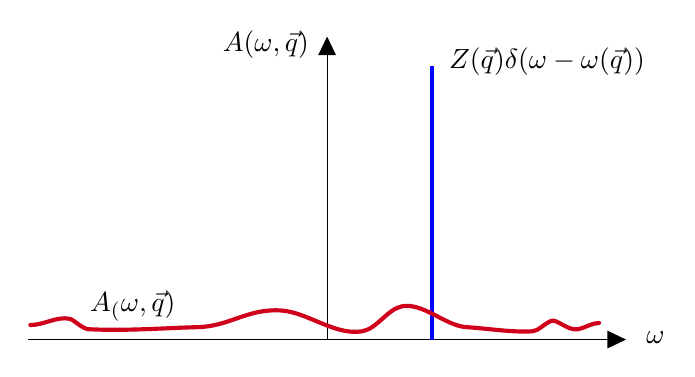
\begin{tikzpicture}[x=0.75pt,y=0.75pt,yscale=-1,xscale=1]
\draw    (94.5,195) -- (379.5,195) ;
\draw [shift={(382.5,195)}, rotate = 180] [fill={rgb, 255:red, 0; green, 0; blue, 0 }  ][line width=0.08]  [draw opacity=0] (8.93,-4.29) -- (0,0) -- (8.93,4.29) -- cycle    ;
\draw    (238.5,195) -- (238.5,52) ;
\draw [shift={(238.5,49)}, rotate = 450] [fill={rgb, 255:red, 0; green, 0; blue, 0 }  ][line width=0.08]  [draw opacity=0] (8.93,-4.29) -- (0,0) -- (8.93,4.29) -- cycle    ;
\draw [color=blue  ,draw opacity=1 ][line width=1.5]    (289,63) -- (289,195) ;
\draw  [color={rgb, 255:red, 208; green, 2; blue, 27 }  ,draw opacity=1 ][line width=1.5] [line join = round][line cap = round] (95.5,188) .. controls (102.23,188) and (108.09,183.72) .. (114.5,185) .. controls (116.33,185.37) and (120.65,189.85) .. (123.5,190) .. controls (141.15,190.93) and (158.84,189.48) .. (176.5,189) .. controls (191.61,188.59) and (200.37,179.85) .. (216.5,181) .. controls (229.23,181.91) and (242.27,193.21) .. (255.5,191) .. controls (262.38,189.85) and (267.57,180.39) .. (274.5,179) .. controls (284.54,176.99) and (295.68,188.42) .. (305.5,189) .. controls (315,189.56) and (327.9,191.69) .. (337.5,191) .. controls (340.48,190.79) and (342.95,187.42) .. (346.5,186) .. controls (349.17,184.93) and (354.56,190.99) .. (359.5,190) .. controls (362.91,189.32) and (366.02,187) .. (369.5,187) ;
\draw (296,53) node [anchor=north west][inner sep=0.75pt]    {$Z(\vec{q}) \delta (\omega-\omega(\vec q))$};
\draw (187,45) node [anchor=north west][inner sep=0.75pt]    {$A( \omega ,\vec q)$};
\draw (391,190) node [anchor=north west][inner sep=0.75pt]    {$\omega$};
\draw (123,170) node [anchor=north west][inner sep=0.75pt]    {$A_\tinc( \omega ,\vec q)$};
\end{tikzpicture}}
\caption{One-dimensional pictorially representation of the function $A( \omega ,\vec q)$ for a stable particle.}
\label{fig:sharp_behav_A_spect_func}
\end{figure}
%
\noindent
Just notice that since $A(\omega,\vec q)$ has an explicitly physical meaning as probability density, the plot shown in Fig.~\ref{fig:sharp_behav_A_spect_func} can be obtained directly in experiments, up to experimental uncertainties which turn the $\delta$-function into a smooth but very localized function. 

From the sum rule we get
\begin{eq}
	1=\int\de\omega\,A(\omega, \vec q)=Z(\vec q)+\underbrace{\int\de\omega\,A_\tinc(\omega, \vec q)}_{\geq 0}
\end{eq}
which implies
\begin{eq}
	0\leq Z(\vec q)\leq1
\end{eq}

Notice that the case $Z(\vec q)=1$ the theory is free, indeed for a free particle $A(\omega, \vec q)=\delta(\omega-\omega(\vec q))$. Our problem is that, as we'll see, is very difficult to satisfy $0\leq Z<1$ in an interacting situation. 

%%%%%%%%%%%%%%%%%%%%%%%
%%%%%%%% LECTURE 6 %%%%%%%%
%%%%%%%%%%%%%%%%%%%%%%%

We can weaken a little the above requirement of a stable particle excitation: let's see what happen if we do not have a stable particle but a long-life resonance (i.e. a particle with a lifetime large respect to the typical time of the system). The $\delta$-function in eq.~\eqref{eq:stable_1_particle_term_in_spec_func} can be rewritten as
\begin{eq}
	\delta(\omega-\omega(\vec q))\quad\mapsto\quad \frac1\pi \Im\frac1{\omega-\omega(\vec q)+i\delta}
	\quad\text{where the limit $\delta\to 0^+$ is understood}
\end{eq}
and this implies that the retarded correlator has a pole at $\omega=\omega(\vec q)-i\delta$. Notice that $\delta$ essentially correspond to the inverse lifetime $\inv\tau$ of the particle, hence the limit $\delta\to0^+$ correspond to the infinite lifetime of the particle. 

A resonance is described through a Lorentzian distribution, by replacing the above pole by a complex pole at $\omega=f(\omega, \vec q)$ where $f$ is a complex function with $\Im f(\omega,\vec q)<0$ (in such a way that $A(\omega, \vec q)\geq0$ is satisfied). Then
\begin{eq}
	\Im\frac1{\omega-f(\omega, \vec q)}=\frac{-\Im f(\omega, \vec q)}{(\omega-\Re f(\omega, \vec q))^2+(\Im f(\omega, \vec q))^2}
\end{eq}
where $\omega=\Re f(\omega, \vec q)$ describes the dispersion relation of the unstable particle and $\Im f(\omega, \vec q)$ its inverse lifetime.\todo{Qui penso sia $-\Im f$ l'inverse lifetime, visto che $\Im f<0$.} 

If we take $\Im f(\omega, \vec q)\to0^-$ then $\Im\frac1{\omega-f(\omega,\vec q)}\to\delta(\omega-f(\omega,\vec q))$ \todo{Ci va $\frac1\pi$ da qualche parte?} with dispersion relation $\omega(\vec q)$ solution of the equation $\omega-\Re f(\omega, \vec q)=0$ and we recover the case of a stable particle:
\begin{eq}
	\delta(\omega-f(\omega, \vec q))=\frac{\displaystyle \delta(\omega-\omega(\vec q))}{\displaystyle \left|\pder f\omega(\omega, \vec q)\right|\Big|_{\omega=\omega(\vec q)}}
	=Z(\vec q)\delta(\omega-\omega(\vec q))
\end{eq}
This means that in the case of the resonance we just broaden the $\delta$-function in the spectral function, as shown in fig.~\ref{fig:res_behav_A_spect_func}. 
      
\begin{figure}[H]
\centering
\scalebox{.9}{
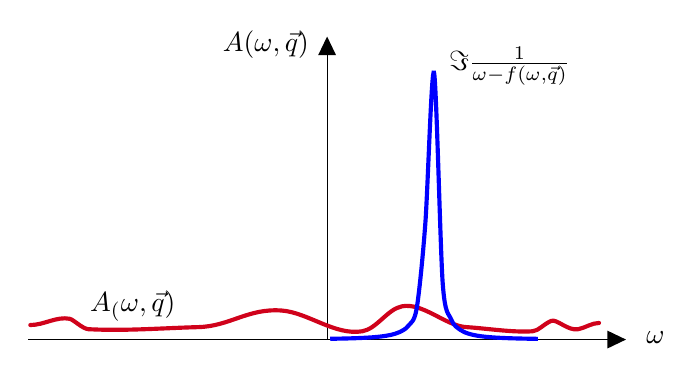
\begin{tikzpicture}[x=0.75pt,y=0.75pt,yscale=-1,xscale=1]
\draw    (94.5,195) -- (379.5,195) ;
\draw [shift={(382.5,195)}, rotate = 180] [fill={rgb, 255:red, 0; green, 0; blue, 0 }  ][line width=0.08]  [draw opacity=0] (8.93,-4.29) -- (0,0) -- (8.93,4.29) -- cycle    ;
\draw    (238.5,195) -- (238.5,52) ;
\draw [shift={(238.5,49)}, rotate = 450] [fill={rgb, 255:red, 0; green, 0; blue, 0 }  ][line width=0.08]  [draw opacity=0] (8.93,-4.29) -- (0,0) -- (8.93,4.29) -- cycle    ;
\draw  [color={rgb, 255:red, 208; green, 2; blue, 27 }  ,draw opacity=1 ][line width=1.5] [line join = round][line cap = round] (95.5,188) .. controls (102.23,188) and (108.09,183.72) .. (114.5,185) .. controls (116.33,185.37) and (120.65,189.85) .. (123.5,190) .. controls (141.15,190.93) and (158.84,189.48) .. (176.5,189) .. controls (191.61,188.59) and (200.37,179.85) .. (216.5,181) .. controls (229.23,181.91) and (242.27,193.21) .. (255.5,191) .. controls (262.38,189.85) and (267.57,180.39) .. (274.5,179) .. controls (284.54,176.99) and (295.68,188.42) .. (305.5,189) .. controls (315,189.56) and (327.9,191.69) .. (337.5,191) .. controls (340.48,190.79) and (342.95,187.42) .. (346.5,186) .. controls (349.17,184.93) and (354.56,190.99) .. (359.5,190) .. controls (362.91,189.32) and (366.02,187) .. (369.5,187) ;
\draw[scale=1, domain=240:340, smooth, variable=\x, blue][line width=1.5] plot (\x,{195-900/((\x-289)*(\x-289)+6)});
\draw (296,53) node [anchor=north west][inner sep=0.75pt]    {$\Im\frac1{\omega-f(\omega, \vec q)}$};
\draw (187,45) node [anchor=north west][inner sep=0.75pt]    {$A( \omega ,\vec q)$};
\draw (391,190) node [anchor=north west][inner sep=0.75pt]    {$\omega$};
\draw (123,170) node [anchor=north west][inner sep=0.75pt]    {$A_\tinc( \omega ,\vec q)$};
\end{tikzpicture}}
\caption{One-dimensional pictorially representation of the function $A( \omega ,\vec q)$ for a unstable particle. The width of the blue peak is proportional to the inverse lifetime $\inv\tau$ of the particle.}
\label{fig:res_behav_A_spect_func}
\end{figure}

Again, provided CCR or CAR (depending on the physical situation) we again have the contstraint\todo{Penso che qui $Z(\vec q)$ vada definito come $\int\de\omega\Im\frac1{\omega-f(\omega, \vec q)}$ }
\begin{eq}\label{eq:bound_Z_spect_repr}
	0\leq Z(\vec q)\leq 1
\end{eq}
hence the constraint applies even if we consider unstable particles.

\section{The incompatibility between CCR and $U^I$}

Let's see what have to do the previous spectral representations with the inconsistency of the perturbation theory as $\epsilon\to0$, first considering the relativistic case.

Let's inspect the relation between $Z$ and asymptotic fields. With the introduction of the infrared cutoff $\epsilon$ (at least in $t$) we got that the free field is related to the interacting field by a unitary operator
\begin{eq}
	\ophi(\vec x,t) =\ueid(t)\ophi_\tin(\vec x, t)\uei(t)
\end{eq}
such that
\begin{eq}
	\ophi(\vec x,t) \xrightarrow[t\to-\infty]{}\ophi_\tin(\vec x,t)
	\tand
	\uei(t)\xrightarrow[t\to-\infty]{}\id
\end{eq}
Let's see if such unitary relation between free and interacting field is possible preserving translational invariance. 

Consider a one particle system, since \todo{Questa affermazione va controllata, non so se è proprio questo il motivo.} $\bra0\ophi_\tin\ophi_\tin\ket0$ has exactly a pole for $q^2=m^2$ we can identify $\bra0\ophi_\tin\ophi_\tin\ket0$ as responsible for the contribution
\begin{eq}\label{eq:contr_A_relativ_case}
	Z\delta(q^2-m^2)\theta(q^0)
\end{eq}
in the spectral function $A(q)$ of $\ophi$, eq.~\eqref{eq:split_spect_func_delta_inc}. We want that $\ophi$ describes an interacting field, so we assume $Z\neq1$ (otherwise $\ophi$ is free), conversely for $\ophi_\tin$ we already know that eq.~\eqref{eq:contr_A_relativ_case} is satisfied for $Z=1$. Therefore it is impossible to satisfy $\ophi \xrightarrow[t\to-\infty]{}\ophi_\tin$, one can at best hope to satisfy $\ophi \xrightarrow[t\to-\infty]{}Z^{1/2}\ophi_\tin$, i.e.
\begin{eq}\label{eq:free_int_unit_rela_Z}
	\ophi(\vec x,t) =Z^{1/2}\ueid(t)\ophi_\tin(\vec x, t)\uei(t)
\end{eq}
which means that $\ophi_\tin$ is related by a unitary transformation to the renormalized field $Z^{-1/2}\ophi$. 

But if $\ophi_\tin$ and $\ophi$ are canonical, i.e. satisfy CCR, then eq.~\eqref{eq:free_int_unit_rela_Z} must be wrong, indeed from eq.~\eqref{eq:free_int_unit_rela_Z} we get
\begin{eq}\label{eq:limit_t_-inf_CCR}
	[\ophi(\vec x,t),\dot\ophi(\vec y,t)]\xrightarrow[t\to-\infty]{}Z[\ophi_\tin(\vec x,t),\dot\ophi_\tin(\vec y,t)]
\end{eq}
but then using CCR for $\ophi_\tin$ and $\ophi$ we get
\begin{eq}\label{eq:inconsistency_CCR_unitary}
	\delta(\vec x -\vec y)
	&\overset{\text{CCR}}=\lim_{x^0\to-\infty}\bra0[\ophi(\vec x,x^0),\dot\ophi(\vec y,y^0)]\ket0\big|_{x^0=y^0}=\\
	&=Z\lim_{x^0\to-\infty}\bra0[\ophi_\tin(\vec x,x^0),\dot\ophi_\tin(\vec y,y^0)]\ket0\big|_{x^0=y^0}\overset{\text{CCR}}=Z\delta(\vec x -\vec y)
\end{eq}
which give $Z=1$, but this is wrong since we assumed that $\ophi$ is interacting. 

\skipline

Notice that the above argument about the inconsistency between CCR and eq.~\eqref{eq:free_int_unit_rela_Z} requires that both $x^0$ and $y^0$ are sent to $-\infty$ simultaneously in eq.~\eqref{eq:limit_t_-inf_CCR}. Conversely it is still possible that $\ophi$ approaches $Z^{1/2}\ophi_\tin$ as $t\to-\infty$ in the weak sense $\ophi \xrightharpoonup[t\to-\infty]{}Z^{1/2}\ophi_\tin$, i.e. in matrix elements: taken a sequence $A_n$ of operators the \emph{weak limit} 
\begin{eq}
	A_n\xrightharpoonup[n\to+\infty]{} A
\end{eq}
means that 
\begin{eq}
	|\langle\psi,(A_n-A)\phi\rangle|\xrightarrow[n\to+\infty]{}0
\end{eq} 
Indeed taken $A_n\rightharpoonup A$ and $B_n\rightharpoonup B$ is not ensured that $A_nB_n\rightharpoonup AB$, therefore $\ophi(x)\xrightharpoonup[x^0\to-\infty]{}Z^{1/2}\ophi_\tin(x)$ and $\dot\ophi(y)\xrightharpoonup[y^0\to-\infty]{}Z^{1/2}\dot\ophi_\tin(y)$ does not imply $[\ophi(x),\dot\ophi(y)]\xrightarrow[x^0,y^0\to-\infty]{}Z[\ophi_\tin(x),\dot\ophi_\tin(y)]$ and eq.~\eqref{eq:limit_t_-inf_CCR} does not hold anymore. Therefore if $\ophi(x)\xrightharpoonup[x^0\to-\infty]{}Z^{1/2}\ophi_\tin(x)$ we don't have any inconsistency between CCR and eq.~\eqref{eq:free_int_unit_rela_Z}.\footnote{More about this fact in \cite[Section 9.2]{Greiner_1996}.}

Notice that LSZ formula uses precisely such weak limit for $t\to-\infty$, so there is no inconstistence with it.\footnote{The derivation of the LSZ formula for the scalar theory can be found in \cite[Section 9.4]{Greiner_1996}.} 

The serious problem arises when in perturbative approach is used the Gell-Mann Low formula, which requires the existence of a unitary operator $U^I=\lim_{\epsilon\to0^+}\uei$ interpolating between $\ophi$ and $\ophi_\tin$, but if $\ophi$ obeys CCR and translation invariance is recovered (i.e. we take the limit $\epsilon\to0^+$) we get from eq.~\eqref{eq:free_int_unit_rela_Z}  that such unitary operator does not exist (in order to get unitarity we should have $Z=1$, which is forbidden if $\ophi$ is interacting).

\section{The Haag's theorem}

\cite[Section 3]{Earman:2005}; \cite[Section 4.5]{Streater:2000}; \cite[Pages 39-40, 95-96]{Strocchi_2013}\\

The important argument from Haag\footnote{Original paper: \cite{Haag:1955}.} proves that the situation does not improve even if we do not require $\ophi$ to be canonical. Except very special non-relativistic cases, the Hilbert space of the free field is disjoint from the Hilbert space of the interacting field (i.e. doesn't exist any unitary operator which maps the states of one Hilbert spaces into the states of the other one). 

\begin{theorem}[{Haag, \cite[Page 8]{Earman:2005}}]
	Assume that the unique translationally invariant state of an interacting scalar QFT with Hilbert space $\hs$ and field $\ophi\in\hs$ is the vacuum $\ket0\in\hs$ \footnote{It is reasonable to assume that the only translationally invariant state should be the vacuum, as the presence of any particle broke translational invariance. This is ensured if the underlying free theory has a mass gap, i.e. all particles of our theory are massive. In general these assumptions does not hold if the free theory has massless particles. See \cite[Section 3]{Earman:2005} for further comments about this fact.} (for lattice theories only discrete translations are considered). Suppose that the Hamiltonian of the theory can be written as $H=H_0+H_I$, with $H_0$ free Hamiltonian. 
	
	Then there is no state $\ket{0_F}\in\hs$ such that $H_0\ket{0_F}=0$ and $H\ket{0_F}\neq0$ i.e. if the interacting Hamiltonian $H$ does not annihilate the vacuum of the free theory $\ket{0_F}$ then $\ket{0_F}$ is not an element of $\hs$ .
\end{theorem}
\begin{proof}
	Let $U(\vec x)$, $\vec x\in\R^d$, be the unitary representation of translations in $\hs$.
	Assume that the Fock vacuum $\ket{0_F}$ of the free theory with Hamiltonian $H_0$ is an element of $\hs$, i.e. $\ket{0_F}\in\hs$ such that $H_0\ket{0_F}=0$. Denote by $a_F(\vec q)$ the annihilation operator of $H_0$ ($F= \text{free}$), then
	\begin{eq}
		U^\dagger(\vec x)a_F(\vec q)U(\vec x)=e^{i\vec q\cdot\vec x}a_F(\vec q)
	\end{eq}
	therefore
	\begin{eq}
		0=U^\dagger(\vec x)a_F(\vec q)\ket{0_F}=U^\dagger(\vec x)a_F(\vec q)U(\vec x)U^\dagger(\vec x)\ket{0_F} = e^{i\vec q\cdot\vec x}a_F(\vec q)U^\dagger(\vec x)\ket{0_F}
	\end{eq}
	and this means that $a_F(\vec q)$ annihilates $U^\dagger(\vec x)\ket{0_F}$, hence $U^\dagger(\vec x)\ket{0_F}$ is translationally invariant. By uniqueness of the translational invariant state $\ket{0_F}=c\ket0$ for some constant $c$ (actually if our states are normalized $c$ is just a phase). Then
	\begin{eq}
		0=H\ket0=(H_0+H_I)c\ket{0_F}=c\,H_I\ket{0_F}
	\end{eq}
	which give us $H_I\ket{0_F}=0$ and $H\ket{0_F}=0$.
\end{proof}

Under some hypothesis, this first version of Haag's theorem proves that the vacuum of the free theory cannot be an element of the Hilbert space of the interacting theory. The relative simplicity of this theorem is purchased at the expense of generality since it appeals to the fact that typical Hamiltonians for interacting fields do not annihilate $\ket{0_F}$, $H\ket{0_F}\neq0$, (\emph{excitations of the vacuum}).\footnote{As an illustration, consider the $\ophi^4$ scalar field in $\R^{3+1}$ with (formal) Hamiltonian
	\begin{eq}
		H=H_0+\lambda\int\de^3x\,:\ophi^4:-\,C
	\end{eq}
where $C$ is a constant $c$-number chosen to give vanishing ground state energy, and $:\quad:$ indicates the Wick normal product. This $H$ will not annihilate the bare vacuum $\ket{0_F}$ since the factor that follows the coupling constat $\lambda$ contains a term with a product of four creation operator $\sim (a^\dagger)^4$ (and there is only one term of this form, so it will not be canceled by another term).} 
	
It was the ambition of the second version of his theorem to dispense with any reference to the particular form of the interacting field Hamiltonian. However, Haag's attempted proof of such general version was found ``inconclusive''. The gap was filled by a pair of theorems presented by Hall and Wightman,\footnote{Original paper: \cite{Hall:1957}} which together constitutes the so called \emph{Haag-Hall-Wightman (HHW) theorem}, which applies to any pair of neutral scalar field.

\begin{theorem}[{HHW Part 1, \cite[Section 3, Thm. 1]{Hall:1957}, \cite[Thm. 4.14]{Streater:2000}}]\label{thm:HHW1}
	Consider two QFTs with scalar fields $\ophi_1$, $\ophi_2$ and Hilbert spaces $\hs_1$, $\hs_2$ and assume that
	\begin{enumerate}[label=(\roman*)]
	\item the Euclidean group $\mathbb E_d$ (roto-traslations) is represented unitarily by $U_1$ and $U_2$ on $\hs_1$ and $\hs_2$ respectively:
	\begin{eq}
		U_j(\vec a,\vec R)\ophi_j(\vec x,t) U_j^\dagger(\vec a, \vec R)=\ophi_j(\vec R\,\vec x+\vec a,t)
	\end{eq}
	\item the representation of the fields is irreducible, i.e. if an operator $\op A$ defined in $\hs_j$ commutes with all the fields $\{\ophi_j\}\subset\hs_j$ then it is a multiple of the identity, $\op A=a\,\id$ for $a\in\C$;
	\item the fields are related at some time $t$ by a unitary transformation $V(t)$
	\begin{eq}\label{eq:HHW-hp-fields}
		\ophi_2(\vec x,t)=V(t)\ophi_1(\vec x,t) V^\dagger(t)
	\end{eq}
	\end{enumerate}
	Then 
	\begin{eq}\label{eq:HHW1_thesis1}
		U_2(\vec a,\vec R)=V(t)U_1(\vec a,\vec R)V^\dagger(t)
	\end{eq}
	Further, if there are unique states $\ket{0_1}$ and $\ket{0_2}$ invariant under $\mathbb E_d$, $U_j(\vec a,\vec R)\ket{0_j}=\ket{0_j}$ for $j=1,2$, then
	\begin{eq}\label{eq:HHW1_thesis2}
		V(t)\ket{0_1}=c\,\ket{0_2} \twith c\in\C
	\end{eq}
	In particular if $\ket{0_j}$, $j=1,2$ are normalized to 1 then $|c|=1$.
\end{theorem}

Notice that this part of the theorem holds also in the non-relativistic case. The operator $V$ is meant to be the unitary operator interpolating between the free and the interacting fields in the Gell-Mann Low formula.

\begin{proof}
	Consider the operator $U_1^\dagger(\vec a,\vec R) V^\dagger(t) U_2(\vec a,\vec R) V(t)$, this commutes with all $\ophi_1\in\hs_1$, indeed:
	\begin{eq}
		&U_1^\dagger(\vec a,\vec R) V^\dagger(t) U_2(\vec a,\vec R) V(t)\ophi_1(\vec x,t)V^\dagger(t)U_2^\dagger(\vec a,\vec R)V(t)U_1(\vec a,\vec R)=\\
		&=U_1^\dagger(\vec a,\vec R) V^\dagger(t) U_2(\vec a,\vec R) \ophi_2(\vec x,t)U_2^\dagger(\vec a,\vec R)V(t)U_1(\vec a,\vec R)=\\
		&=U_1^\dagger(\vec a,\vec R) V^\dagger(t)\ophi_2(\vec R\,\vec x+\vec a,t)V(t)U_1(\vec a,\vec R)=\\
		&=U_1^\dagger(\vec a,\vec R)\ophi_1(\vec R\,\vec x+\vec a,t)U_1(\vec a,\vec R)=\\
		&=U_1^\dagger(\vec a,\vec R)U_1(\vec a,\vec R)\ophi_1(\vec x,t)U_1(\vec a,\vec R)U_1^\dagger(\vec a,\vec R)=\\
		&=\ophi_1(\vec x, t)
	\end{eq}
	which implies
	\begin{eq}
		U_1^\dagger(\vec a,\vec R) V^\dagger(t) U_2(\vec a,\vec R) V(t)\ophi_1(\vec x,t) = \ophi_1(\vec x,t)U_1^\dagger(\vec a,\vec R) V^\dagger(t) U_2(\vec a,\vec R) V(t)
	\end{eq}
	Due to the irreducibility of the representation we get that
	\begin{eq}\label{eq:dfn-omega-HHW}
		U_1^\dagger(\vec a,\vec R) V^\dagger(t) U_2(\vec a,\vec R) V(t) = \omega(\vec a,\vec R)\id
	\end{eq}
	for some complex function $\omega(\vec a,\vec R)$ which depend on the element $(\vec a,\vec R)\in\mathbb E_d$ and then
	\begin{eq}\label{eq:HHW1_proof_eq1}
		\omega(\vec a,\vec R)U_1(\vec a,\vec R)=V^\dagger(t) U_2(\vec a,\vec R) V(t)
	\end{eq}
	Notice that in order to preserve unitarity we must have $|\omega(\vec a,\vec R)|=1$ for all $(\vec a,\vec R)\in\mathbb E_d$. By definition eq.~\eqref{eq:dfn-omega-HHW} $\omega(\vec a,\vec R)$ provides a continuous one-dimensional representation (on $\C$) of a non-compact group ($\mathbb E_d$), and it is a general mathematical result that the unique representation with these properties is the trivial one; hence one may take $\omega(\vec a,\vec R)=1$.  
	
	If there are unique states $\ket{0_j}$ invariant under $\mathbb E_d$, $U_j(\vec a,\vec R)\ket{0_j}=\ket{0_j}$, then from $U_1(\vec a,\vec R)\ket{0_1}=\ket{0_1}$ one gets using eq.~\eqref{eq:HHW1_proof_eq1}
	\begin{eq}
		&V^\dagger(t) U_2(\vec a,\vec R) V(t)\ket{0_1}=\ket{0_1}
	\end{eq}
	and
	\begin{eq}
		&U_2(\vec a,\vec R) V(t)\ket{0_1}=V(t)\ket{0_1}
	\end{eq}
	but the only state in $\hs_2$ invariant under $U_2(\vec a,\vec R) $ is $\ket{0_2}$, therefore we must have
	\begin{eq}
		V(t)\ket{0_1} = c \ket{0_2}
	\end{eq}
	for some constant $c\in\C$, which should be a phase, $|c|=1$, if $\ket{0_1}$ and $\ket{0_2}$ are normalized to 1.
\end{proof}

\begin{corollary}\label{cor:HHW_1}
	For any pair of theories satisfying the hypothesis of theorem \ref{thm:HHW1} the equal time correlation functions of $\ophi_1$ and $\ophi_2$ coincides
	\begin{eq}
		\bra{0_1}\ophi_1(\vec x_1,t)\cdots\ophi_1(\vec x_n,t)\ket{0_1}=\bra{0_2}\ophi_2(\vec x_1,t)\cdots\ophi_2(\vec x_n,t)\ket{0_2}
	\end{eq}
\end{corollary} 
\begin{proof}
	The statement directly follows from eq.~\eqref{eq:HHW-hp-fields} and eq.~\eqref{eq:HHW1_thesis2}.
\end{proof}

In principle an operator $V$ satisfying the hypothesis of Gell-Mann Low formula can still exists, and corollary \ref{cor:HHW_1} still admits different dynamics for $\ophi_1$ and $\ophi_2$ since it applies only for equal time correlators. As we consider correlators at different time one should use time evolution operators involving the Hamiltonian, and no useful conclusion can be stated at this point if there is no vacuum polarization. We need one more result, which however works only in the relativistic case:

\begin{theorem}[{HHW Part 2, \cite[Section 3, Thm. 2]{Hall:1957}, \cite[Thm. 4.16]{Streater:2000}}]\label{thm:HHW2}
	Under the hypothesis of theorem \ref{thm:HHW1} assume further that the (covering of the) restricted Poincaré group $\poinc$ is represented unitarily by $U_1$ and $U_2$ on $\hs_1$ and $\hs_2$ respectively, i.e.
	\begin{eq}
		U_j(\Lambda, a)\ophi_j(x) U_j^\dagger(\Lambda, a)=\ophi_j(\Lambda\, x+ a)
	\end{eq}
	Then
	\begin{eq}
		\bra{0_1}\ophi_1(x)\ophi_1(y)\ket{0_1}=\bra{0_2}\ophi_2(x)\ophi_2(y)\ket{0_2}
	\end{eq}
	and if $\ophi_1$ is a free field of mass $m>0$, then $\ophi_2$ is a free field of mass $m>0$ too.
\end{theorem}
\begin{proof}
	The proof is much more involved than the previous one, since requires a preliminary result of R. Jost and B. Schroer, which can be found in \cite[Thm. 4.15]{Streater:2000}. We just sketch the argument for the proof: by Poincaré covariance through a boost transformation we can bring any two points in the space-time to equal time, in such a way that corollary \ref{cor:HHW_1} applies. Then the correlator we obtained can be extended to the initial points by analiticity, preserving the value of $Z$ and the position of the pole in the Källen-Lehmann representation. This is enough to prove the statement of the theorem.  
\end{proof}

The immediate consequence of the latter is that, if the hypothesis holds, any interacting theory related to a free one by a unitary transformation is actually free. The conclusion that all the fields are free is unacceptable because the intention is to represent an interacting field, therefore at least one of the assumptions of the theorem must be dropped. An obvious candidate is the assumption that at some $t$ there exists a unitary transformation $V(t)$ relating the fields. Therefore the Heisenberg dynamics of the interacting field does not exist in the Hilbert space of the free field, but requires a different Hilbert space, inequivalent to the free one.  

%%%%%%%%%%%%%%%%%%%%%%%
%%%%%%%% LECTURE 7 %%%%%%%%
%%%%%%%%%%%%%%%%%%%%%%%

The second part of the HHW theorem applies only to relativistic QFT, nevertheless the unitary operator $U^I$ interpolating between free and interacting fields does not exists also in most of the non-relativistic QFT, except for very special cases. Therefore almost always the perturbative approach is not mathematically consistent. 

\section{Ultraviolet singularities and canonical quantization}

\cite[Section 2.4]{Strocchi_2013}\\

Consider a RQFT such that $Z=0$ (recall that $Z$ is the constant connecting the renormalized and the free field, $\phi\xrightarrow[t\to-\infty]{}Z^{1/2}\ophi_\tin$, $\ophi_\tren:=Z^{-1/2}\ophi\xrightarrow[t\to-\infty]{}\ophi_\tin$) as in the case of perturbation theory, where one usually gets
\begin{eq}
	Z=1-\lambda\infty\sim\frac1{1+\lambda\infty}=0
\end{eq}
where $\infty$ simply denotes some divergent quantity which has been removed through the renormalization procedure. Then at fixed time the field itself does not exist as an operator. In order to have a well defined operator, one needs to smear $\ophi(x)$ not only in space
\begin{eq}
	\ophi(x^0,f)=\int\de^3x\,f(\vec x)\ophi(x^0,\vec x)
\end{eq}
 but also in time
 \begin{eq}
	\ophi(g)=\int\de^4x\,g(x)\ophi(x)
\end{eq}
Indeed suppose that $\ophi$ is the Heisenberg interacting field, and suppose that it is well defined at fixed time $t$, then according to Källen-Lehmann representation (recall eq.~\eqref{eq:KL_repr_CCR_int}) we get
\begin{eq}
	\bra0[\ophi(t,\vec x),\dot\ophi(t,\vec y)]\ket0=c\,i\delta(\vec x-\vec y)
\end{eq} 
for a constant $c$, which may diverge and in general is strictly positive. Therefore the ``renormalized'' field $\ophi_\tren=Z^{-1/2}\ophi$ which approaches weakly $\ophi_\tin$ as $t\to-\infty$, satisfies
\begin{eq}
	\bra0[\ophi_\tren(t,\vec x),\dot\ophi_\tren(t,\vec y)]\ket0=c\frac iZ\delta(\vec x-\vec y)
\end{eq}
Clearly if $Z=0$ this expression is ill-defined (recall that usually $c>0$), but no assumption has been made except that $\ophi$ is well defined at fixed time, hence if $Z=0$ this assumption should be wrong, i.e. the renormalized field cannot be defined at fixed time. A Schrödinger picture requires that we have a definite state at a fixed time, hence we also proved that it is impossible to defined a picture of dynamics using Schrödinger idea if $Z=0$. 

\end{document}